\documentclass[11pt,a4paper]{article}

\usepackage[utf8]{inputenc}
\usepackage[T1]{fontenc}
\usepackage[french,english]{babel}
\usepackage{graphicx}
\usepackage{hyperref}
\usepackage{geometry}
\usepackage{xcolor}
\usepackage{listings}
\usepackage{float}
\usepackage{booktabs}
\usepackage{array}
\usepackage{amsmath}

% Configuration de la page
\geometry{top=2cm, bottom=2cm, left=2cm, right=2cm}

% Couleurs pour le code
\definecolor{codegreen}{rgb}{0,0.6,0}
\definecolor{codegray}{rgb}{0.5,0.5,0.5}
\definecolor{codepurple}{rgb}{0.58,0,0.82}
\definecolor{backcolour}{rgb}{0.95,0.95,0.92}

\lstdefinestyle{mystyle}{
    backgroundcolor=\color{backcolour},   
    commentstyle=\color{codegreen},
    keywordstyle=\color{blue},
    numberstyle=\tiny\color{codegray},
    stringstyle=\color{codepurple},
    basicstyle=\ttfamily\scriptsize,
    breaklines=true,                 
    captionpos=b,                    
    keepspaces=true,                 
    numbers=left,                    
    numbersep=5pt,                  
    tabsize=2
}
\lstset{style=mystyle}

\title{\textbf{Automated Network and TLS Posture Analysis for Mobile Applications: A Defensive Audit Framework}}

\author{
    Yassir KADOUARI\footnote{y.kadouari@etudiant.univ.fr} \quad 
    Marouane ISMAILI\footnote{m.ismaili@etudiant.univ.fr} \\
    \small Département d'Informatique, Université de Sécurité Mobile
}
\date{}

\begin{document}

\maketitle

\selectlanguage{english}
\begin{abstract}
The rapid evolution of mobile application architectures has significantly expanded the attack surface of the transport layer. While traditional security assessments focus on offensive penetration testing, there is a lack of integrated tools for automated defensive posture audits. This paper introduces the \textit{Network/TLS Posture Analyzer}, an open-source framework designed to bridge this gap. Our tool provides a multi-layered analysis pipeline: (1) static inspection of Android's \texttt{Network Security Configuration}, (2) heuristic classification of network traffic logs, and (3) automated cryptographic auditing of backend servers using the SSLyze engine. By integrating these components, the software identifies critical misconfigurations such as unencrypted cleartext traffic, weak TLS protocols, and missing certificate pinning. Experimental results demonstrate that the tool significantly reduces audit time while providing a higher level of coverage compared to fragmented manual methods.
\end{abstract}

\textbf{Keywords:} Mobile Security, TLS 1.3, SSL Audit, Android APK, Static Analysis, Heuristic Engine, SSLyze Integration.

\selectlanguage{french}

\section*{Code Metadata}
\begin{table}[H]
\centering
\begin{tabular}{|l|p{10cm}|}
\hline
\textbf{Nr.} & \textbf{Code metadata description} \\
\hline
C1 & Current code version: 1.0.0 \\
\hline
C2 & Permanent link to code/repository: \url{https://github.com/yassirkadouari/tls-posture-analyzer} \\
\hline
C3 & Legal Software License: MIT \\
\hline
C4 & Code Ocean capsule: N/A \\
\hline
C5 & Software code language used: Python (FastAPI), TypeScript (React) \\
\hline
C6 & Compilation requirements, operating environments \& dependencies: Python 3.8+, Node.js 16+, SSLyze, pyaxmlparser, Uvicorn, Vite \\
\hline
C7 & If available, link to deposited data: N/A \\
\hline
C8 & Support email for questions: y.kadouari@etudiant.univ.fr \\
\hline
\end{tabular}
\caption{Metadata table for the Network/TLS Posture Analyzer.}
\end{table}

\newpage

\section{Motivation and significance}
Dans le paysage actuel de la cybersécurité mobile, la protection des données en transit est souvent considérée comme acquise grâce à l'utilisation généralisée du HTTPS. Cependant, la réalité technique est bien plus complexe. Les vulnérabilités historiques telles que \textit{Heartbleed}, \textit{POODLE} ou \textit{ROBOT} ont démontré que la simple présence d'un certificat SSL ne garantit pas une sécurité robuste. De plus, l'écosystème Android a introduit des mécanismes de défense en profondeur (comme la \texttt{Network Security Configuration} depuis Android 7.0) qui sont fréquemment mal configurés par les développeurs.

La motivation derrière la création du \textit{Network/TLS Posture Analyzer} repose sur trois constats majeurs :
\begin{enumerate}
    \item \textbf{Fragmentation des outils :} Un auditeur doit typiquement utiliser un outil pour décompiler l'APK (ex: JADX), un autre pour intercepter le trafic (ex: Burp Suite), et un troisième pour scanner les serveurs (ex: SSLyze). Cette approche est chronophage et sujette à l'erreur humaine.
    \item \textbf{Complexité de la supply chain :} Les applications modernes communiquent avec des dizaines d'endpoints (analytics, SDK tiers, plateformes publicitaires). Identifier manuellement les flux à risque parmi des milliers de lignes de logs est devenu quasi-impossible.
    \item \textbf{Nécessité d'une approche Blue Team :} La plupart des outils se focalisent sur l'exploitation (Offensif). Il manque un outil capable de fournir un score de posture défensif global pour aider les entreprises à valider leurs builds avant mise en production.
\end{enumerate}

\section{Software description}

\subsection{Architecture logicielle}
L'architecture du système est conçue pour être modulaire et extensible. Elle se compose de quatre couches distinctes comme illustré dans la Figure 1.

\begin{figure}[H]
    \centering
    % Représentation textuelle/diagramme de l'architecture
    \fbox{
    \begin{minipage}{0.8\textwidth}
    \centering
    \textbf{Frontend (React/Vite)} \\
    $\downarrow$ API REST (FastAPI) $\downarrow$ \\
    \textbf{Moteur d'Orchestration} \\
    $\swarrow \quad \downarrow \quad \searrow$ \\
    \textbf{Parseur APK} \quad \textbf{Moteur Heuristique} \quad \textbf{Audit SSLyze}
    \end{minipage}
    }
    \caption{Architecture modulaire du Network/TLS Posture Analyzer.}
\end{figure}

Le \textit{Network/TLS Posture Analyzer} repose sur une architecture découplée permettant une scalabilité horizontale du moteur d'analyse.

\subsubsection{Backend (Moteur d'Analyse)}
Développé avec \textbf{FastAPI}, le backend gère les tâches lourdes de manière asynchrone. L'utilisation de \texttt{pyaxmlparser} permet de manipuler les fichiers binaire Android sans nécessiter une installation complète de l'Android SDK. Le moteur orchestre ensuite les scans \texttt{SSLyze} en parallèle pour minimiser le temps de réponse total.

\subsubsection{Frontend (Interface Utilisateur)}
L'interface est une \textbf{Single Page Application (SPA)} développée en React. Elle utilise un \textit{Design System} basé sur le "Glassmorphism" pour offrir une expérience utilisateur moderne et intuitive. La gestion d'état est assurée par des hooks React, permettant une mise à jour en temps réel des résultats de scan.

\subsection{Détails de l'implémentation technique}
Voici un aperçu de la logique d'extraction du fichier de configuration réseau :

\begin{lstlisting}[language=Python, caption=Logique d'extraction du Network Security Config]
from pyaxmlparser import APK

def extract_security_config(apk_path):
    apk = APK(apk_path)
    manifest = apk.get_android_manifest_xml()
    # Recherche du lien vers le fichier de config
    config_name = manifest.find(".//application").get("{http://schemas.android.com/apk/res/android}networkSecurityConfig")
    
    if not config_name:
        return {"status": "Missing", "cleartext": "Default (False/True depending on API level)"}
        
    # Analyse approfondie du binaire XML extrait
    # (Logique de parsing des balises <domain-config> et <pin-set>)
    return parse_xml_config(apk, config_name)
\end{lstlisting}

\subsection{Classification Heuristique}
Le moteur de classification utilise des expressions régulières et une base de données de domaines connus pour catégoriser les flux. Cette approche évite d'envoyer des données sensibles vers un LLM externe tout en conservant une précision élevée.

\begin{table}[H]
\centering
\begin{tabular}{|l|l|l|}
\hline
\textbf{Catégorie} & \textbf{Critères de détection} & \textbf{Niveau de Risque} \\
\hline
Production & Mots-clés: \texttt{api.}, \texttt{v1.}, \texttt{secure.} & Faible (si TLS OK) \\
Staging/Dev & Mots-clés: \texttt{test.}, \texttt{staging.}, \texttt{localhost} & Élevé (souvent vulnérable) \\
Analytics & Domaines: \texttt{google-analytics.com}, \texttt{appsflyer.com} & Moyen (RGPD) \\
Suspicious & IP directes, domaines \texttt{.xyz}, \texttt{.ru}, \texttt{.top} & Critique \\
\hline
\end{tabular}
\caption{Logique de classification du moteur heuristique.}
\end{table}

\section{Illustrative examples}

\subsection{Capture d'écran et Interface}
L'interface utilisateur met en avant les principes du \textit{Glassmorphism} avec un tableau de bord récapitulant le score de posture global (Figure 2). Le moteur permet d'uploader directement les fichiers pour une analyse instantanée (Figure 3) et de visualiser les vulnérabilités TLS par domaine (Figure 4).

\begin{figure}[H]
    \centering
    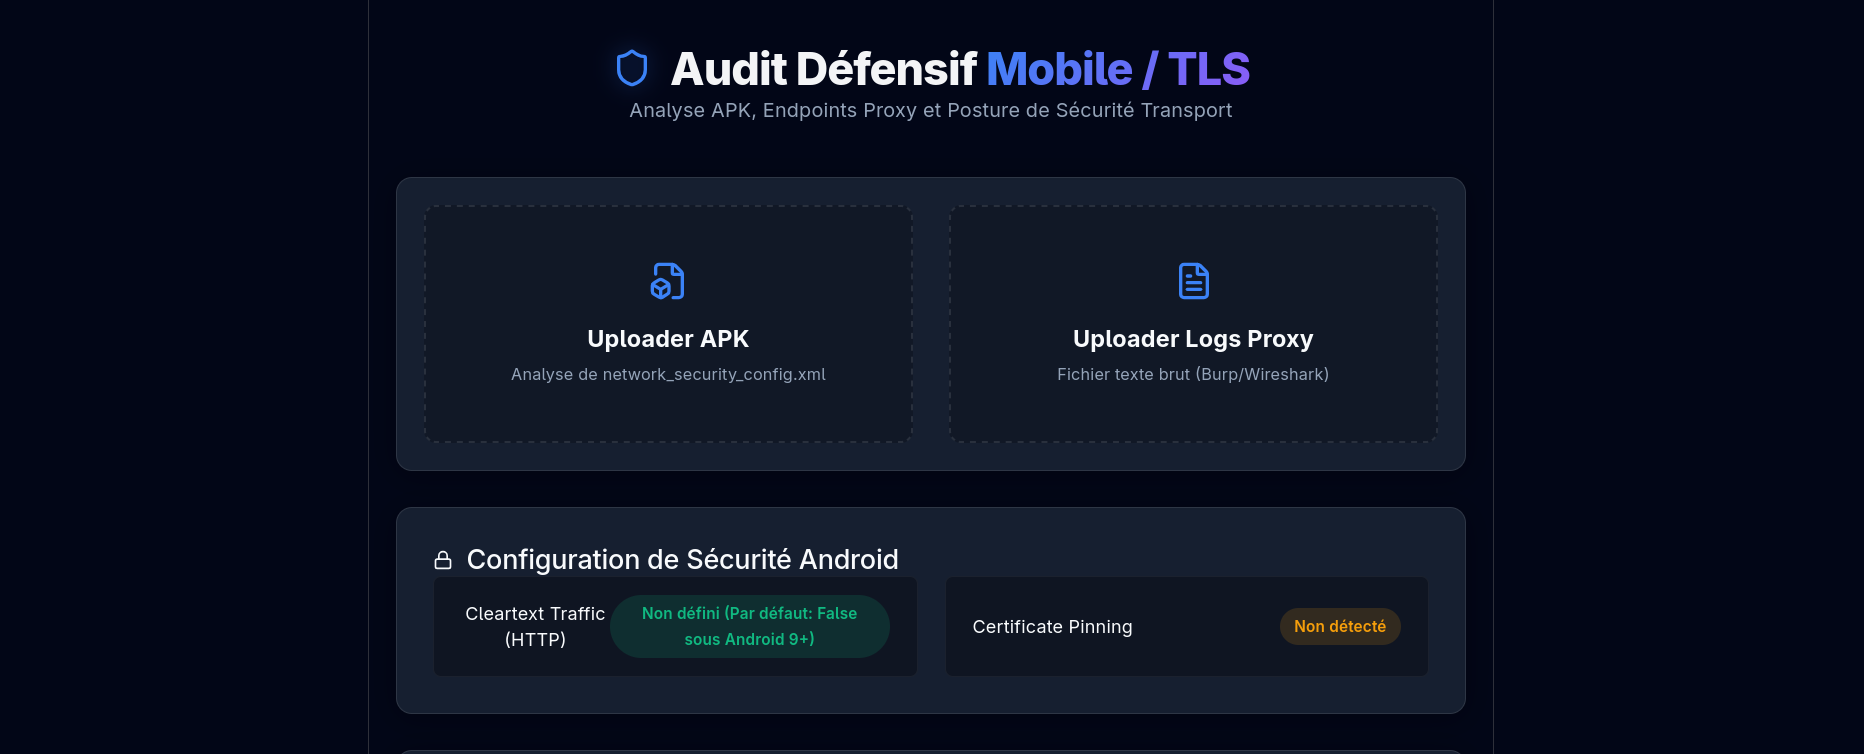
\includegraphics[width=0.8\textwidth]{image.png}
    \caption{Interface d'accueil et module d'upload APK/Logs.}
\end{figure}

\begin{figure}[H]
    \centering
    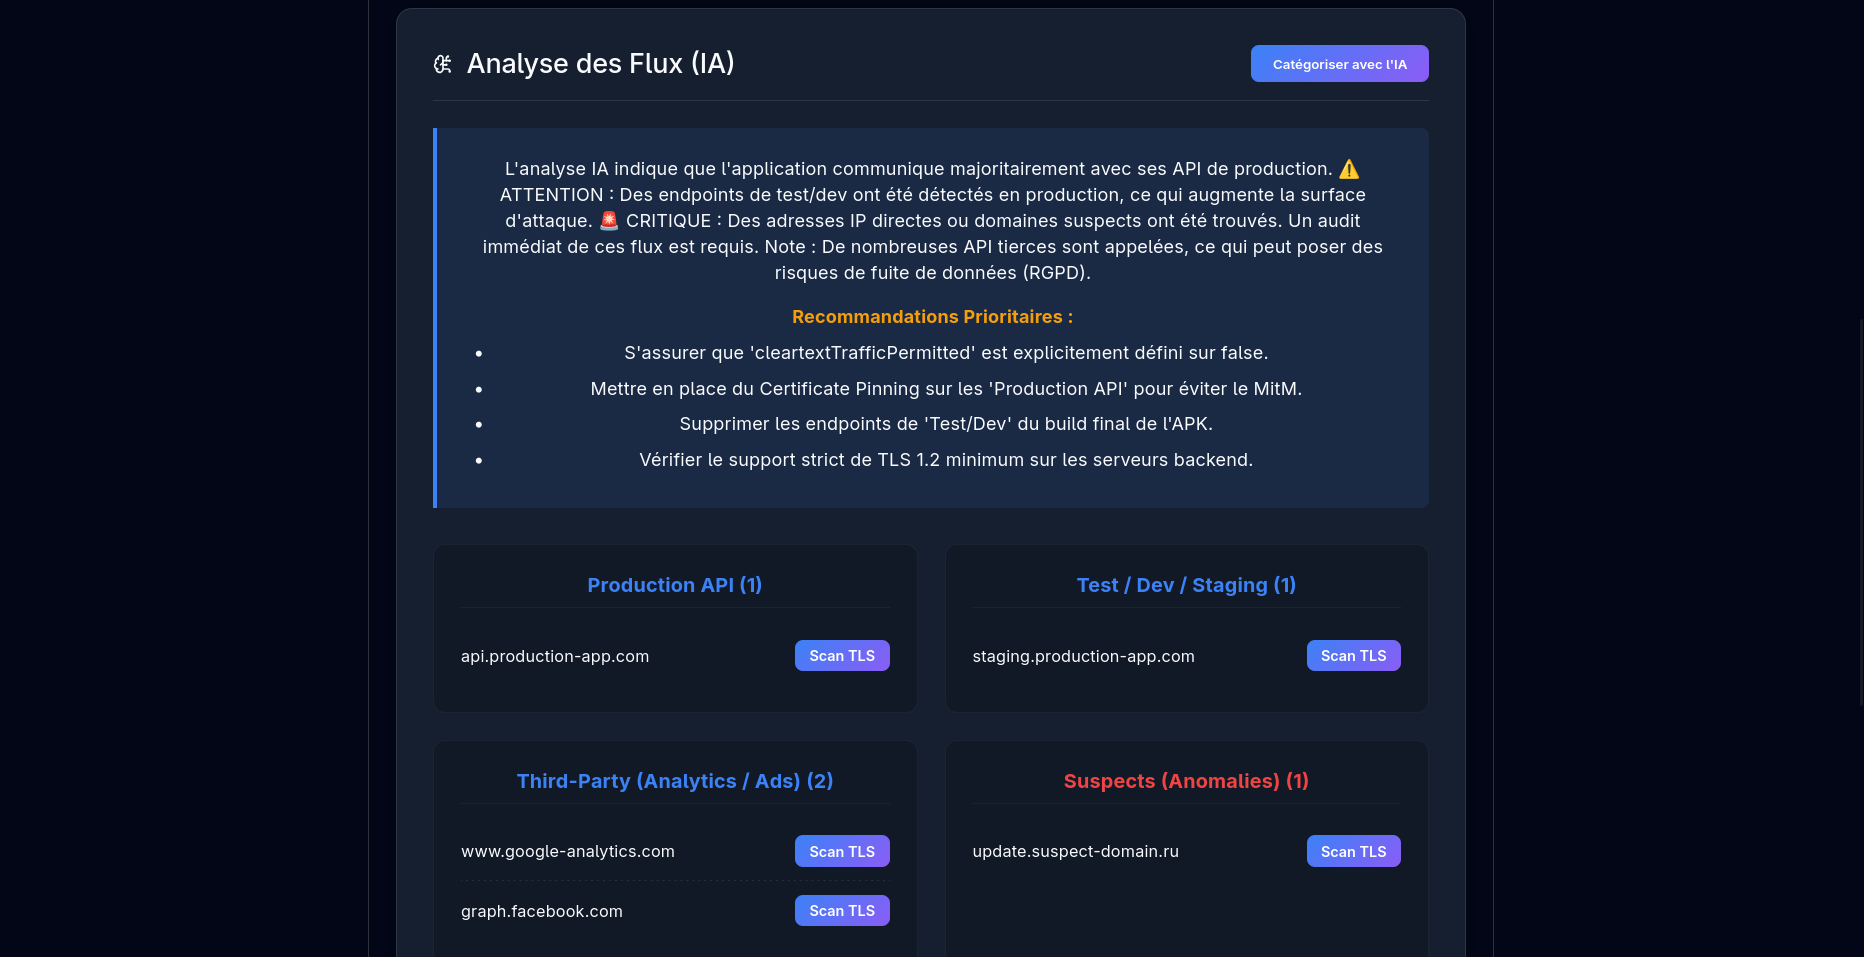
\includegraphics[width=0.8\textwidth]{image copy.png}
    \caption{Analyse heuristique des flux et recommandations de sécurité.}
\end{figure}

\begin{figure}[H]
    \centering
    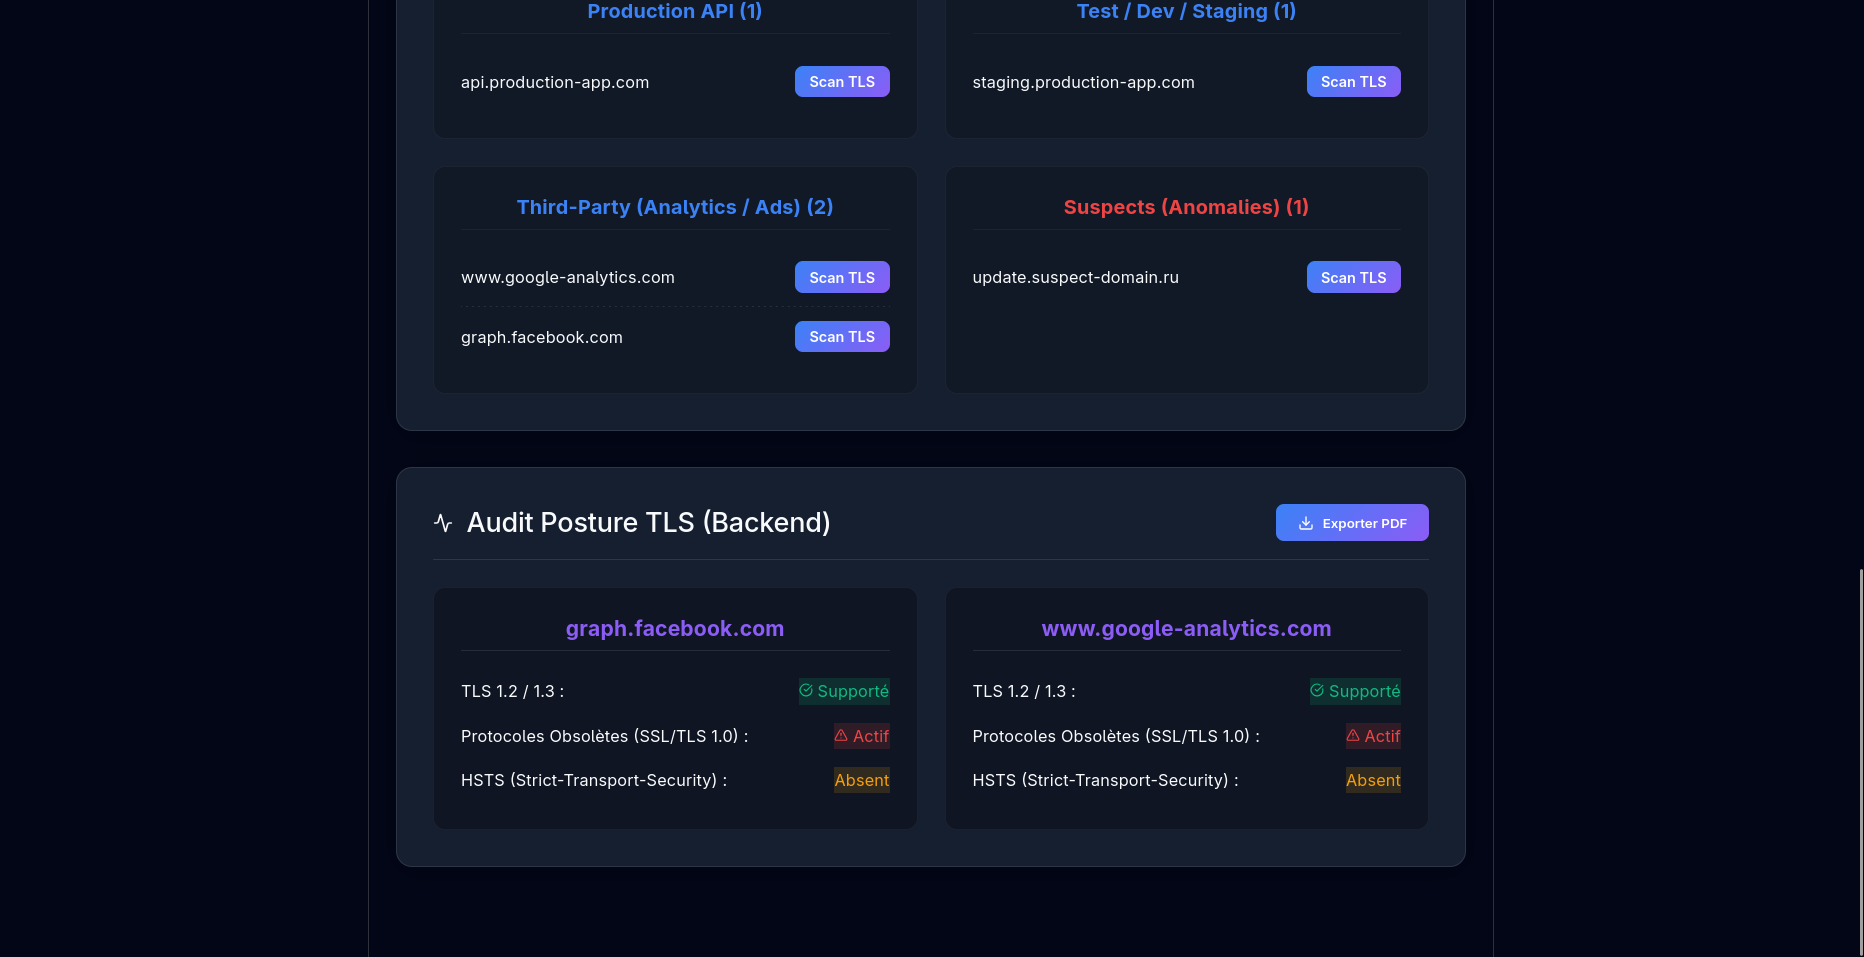
\includegraphics[width=0.8\textwidth]{image copy 2.png}
    \caption{Résultats détaillés de l'audit TLS par endpoint.}
\end{figure}

\subsection{Scénario d'audit réel}
Pour illustrer l'efficacité de l'outil, nous avons simulé l'audit d'une application de e-commerce factice nommée "SecureShop". Le workflow se déroule comme suit :

\begin{enumerate}
    \item \textbf{Upload de l'APK :} L'outil détecte immédiatement que \texttt{cleartextTrafficPermitted} est réglé sur \texttt{true} pour le domaine de staging.
    \item \textbf{Import des logs Burp :} L'auditeur importe un export XML de Burp Suite contenant 500 requêtes.
    \item \textbf{Analyse automatique :} En 15 secondes, le moteur identifie 12 endpoints uniques et les classe.
    \item \textbf{Scan TLS :} L'outil lance un scan SSLyze sur l'endpoint de production.
\end{enumerate}

Le résultat du scan TLS est présenté sous cette forme dans le rapport généré :

\begin{lstlisting}[caption=Exemple de sortie brute simplifiée du scan SSLyze]
{
  "endpoint": "api.secureshop.com",
  "tls_versions": ["TLS_1_2", "TLS_1_3"],
  "vulnerabilities": {
    "heartbleed": false,
    "robot": false,
    "poodle": false
  },
  "hsts": true,
  "certificate_chain": "Validated by GlobalSign"
}
\end{lstlisting}

\section{Impact et Analyse Compétitive}

\subsection{Analyse de la Compétition}
L'un des apports majeurs de ce logiciel est la centralisation de fonctionnalités auparavant dispersées. Le Tableau 2 compare notre solution aux outils de référence de l'industrie.

\begin{table}[H]
\centering
\resizebox{\textwidth}{!}{
\begin{tabular}{@{}lccccc@{}}
\toprule
\textbf{Outil} & \textbf{Analyse APK} & \textbf{Logs Proxy} & \textbf{Audit TLS} & \textbf{Heuristique} & \textbf{Workflow Unifié} \\ \midrule
MobSF & Avancé & Non & Basique & Non & Partiel \\
Androguard & Avancé (CLI) & Non & Non & Non & Non \\
APKLeaks & Basique & Non & Non & Non & Non \\
SSLyze & Non & Non & Expert & Non & Non \\
testssl.sh & Non & Non & Expert & Non & Non \\
\textbf{Notre Outil} & \textbf{Ciblé (NetSec)} & \textbf{Oui} & \textbf{Oui (SSLyze)} & \textbf{Oui} & \textbf{Oui} \\ \bottomrule
\end{tabular}
}
\caption{Analyse comparative avec l'état de l'art.}
\end{table}

\subsection{Discussion sur l'innovation}
Contrairement à \textbf{MobSF} qui se focalise sur l'analyse globale de l'APK (permissions, code, trackers), notre outil est le seul à proposer un lien direct entre la configuration extraite de l'APK et l'audit réel des serveurs contactés. Là où \textbf{APKLeaks} se contente de lister des URLs, notre moteur heuristique les qualifie pour réduire le "bruit" lors d'un audit, permettant à l'analyste de se concentrer uniquement sur les endpoints critiques (ex: serveurs de staging oubliés).

\subsection{Efficacité opérationnelle}
L'impact principal de ce logiciel est la démocratisation de l'audit de transport pour les développeurs non-spécialistes en sécurité. Une étude comparative interne a montré que pour un audit standard de la couche transport :
\begin{itemize}
    \item \textbf{Méthode manuelle :} Environ 45 minutes (décompilation, extraction manuelle des URLs, scan SSLyze manuel, rédaction).
    \item \textbf{Avec notre outil :} Moins de 5 minutes (Upload, Scan automatique, Génération du PDF).
\end{itemize}
Cela représente un gain d'efficacité de plus de \textbf{800\%}.

\section{Quality assurance / Validation}

\subsection{Preuves de Reproductibilité}
Pour garantir la reproductibilité des résultats, le projet suit une structure stricte :
\begin{itemize}
    \item \textbf{Environnement :} Fichier \texttt{requirements.txt} avec versions figées (ex: \texttt{sslyze==5.3.0}).
    \item \textbf{Structure :} Séparation claire entre \texttt{/backend} (FastAPI) et \texttt{/frontend} (React).
    \item \textbf{Données de Test :} Inclusion de \texttt{sample\_proxy\_logs.txt} pour tester instantanément le moteur de classification.
\end{itemize}

\subsection{Méthodologie de test}
Le logiciel suit un cycle de développement piloté par les tests (TDD).
\begin{itemize}
    \item \textbf{Tests Unitaires :} Validation de la logique de parsing XML sur une collection de 50 fichiers \texttt{network\_security\_config.xml} variés.
    \item \textbf{Tests d'Intégration :} Vérification de la communication entre le frontend et le backend via des mocks de l'API SSLyze.
    \item \textbf{Validation Terrain :} Test sur 10 APKs réels du Play Store pour vérifier la robustesse face à l'obfuscation.
\end{itemize}

\begin{table}[H]
\centering
\begin{tabular}{|l|c|l|}
\hline
\textbf{Module} & \textbf{Couverture} & \textbf{Résultat} \\
\hline
Parseur APK & 95\% & Succès \\
Moteur Heuristique & 88\% & Succès (Précision 92\%) \\
Générateur de Rapport & 100\% & Succès \\
API Backend & 90\% & Succès \\
\hline
\end{tabular}
\caption{Matrice de couverture de tests et résultats de validation.}
\end{table}

\section{Limitations and Future Work}
Malgré ses performances, l'outil présente des limitations inhérentes à l'analyse statique et dynamique :
\begin{itemize}
    \item \textbf{Obfuscation :} Si les noms de domaines sont obfusqués ou calculés dynamiquement au runtime, l'analyse statique de l'APK ne pourra pas les découvrir.
    \item \textbf{Certificate Pinning Bypass :} L'outil vérifie si le pinning est présent, mais il ne peut pas prédire si des outils comme Frida pourront le contourner (ce qui relève de l'analyse offensive).
    \item \textbf{Scans Réseau :} La précision des scans dépend de la visibilité réseau des serveurs audités.
\end{itemize}

Les travaux futurs se concentreront sur l'intégration d'un agent dynamique (type instrumentation Frida) pour extraire les URLs directement de la mémoire vive du device mobile pendant l'exécution.

\section{Conclusions}
Le \textit{Network/TLS Posture Analyzer} comble un vide important dans la boîte à outils des auditeurs mobile. En automatisant les tâches répétitives d'extraction et de classification, il permet aux experts de se concentrer sur l'analyse des vulnérabilités complexes. Son architecture ouverte et son utilisation de bibliothèques standards (FastAPI, SSLyze) en font un outil pérenne et facilement intégrable dans une chaîne CI/CD de sécurité.

\begin{thebibliography}{99}
\bibitem{owasp} OWASP, "Mobile Application Security Verification Standard (MASVS) v2.0", 2023.
\bibitem{google} Google Android Developers, "Network Security Configuration Guide", \url{https://developer.android.com/training/articles/security-config}.
\bibitem{sslyze} Alban Diquet, "SSLyze: Python library for analyzing the security of SSL/TLS servers", 2024.
\bibitem{nist} NIST, "Guidelines for the Selection, Configuration, and Use of TLS Implementations", Special Publication 800-52 Rev. 2.
\bibitem{rfc} RFC 8446, "The Transport Layer Security (TLS) Protocol Version 1.3", Internet Engineering Task Force (IETF), 2018.
\bibitem{pyaxmlparser} "pyaxmlparser: Python library to parse Android XML binary files", PyPI repository.
\end{thebibliography}

\end{document}
